\documentclass[
  12pt,
  DIV = 8,
  toc = bibliography,
  titlepage,
  parskip=half
]{scrreprt}

\usepackage{lib/hsa_style}
\usepackage{lib/code}
\usepackage{lib/commands}

\hypersetup{pdfauthor={Roman Kolesnikov},
  pdftitle={Abschlussdokumentation \- Chatter},
  pdfsubject={Abschlussdokumentation \- Chatter},
  pdfkeywords={},
  pdfproducer={LaTeX},
  pdfcreator={pdfLaTeX}
}

\renewcommand{\AutorName}            {Roman Kolesnikov}
\renewcommand{\AutorMatrikelnummer}  {2173133}
\renewcommand{\AutorStrasse}         {Kolbergstr.~18}
\renewcommand{\AutorPLZOrt}          {86167 Augsburg}
\renewcommand{\AutorEMail}           {roman.kolesnikov1@hs-augsburg.de}
\renewcommand{\AutorTelefon}         {+49\,17645624204}
\renewcommand{\AutorOrtUnterschrift} {Augsburg}
\renewcommand{\ArbeitThema}          {Chatter -- Chatplattform für Teams}
\renewcommand{\Studiengang}          {Informatik (M.Sc.)}

\renewcommand{\ArbeitTyp}{Abschlussdokumentation}

\renewcommand{\Abschluss}{Bachelor of Science}

% \renewcommand{\FakultaetTelefon} {}
% \renewcommand{\FakultaetEMail}   {}

\renewcommand{\DatumAbgabe}        {\today}
% \renewcommand{\DatumThemenvergabe} {20.\ Oktober 2022}
\renewcommand{\DatumVerteidigung}  {\today} \booltrue{Verteidigung}

\renewcommand{\NonDisclosure} {Nein}
\renewcommand{\Erstpruefer}        {Dipl.-Inf.~(FH), Dipl.-Designer~(FH),\\ & & M.A. Erich Seifert}
% \renewcommand{\Zweitpruefer}       {Dipl.-Inf.~(FH), Dipl.-Designer~(FH),\\ & & M.A. Erich Seifert} \booltrue{Zweitpruefer}
\renewcommand{\HochschuleName}     {Technische Hochschule Augsburg}
\renewcommand{\HochschuleStrasse}  {An der Hochschule 1}
\renewcommand{\HochschulePLZOrt}   {D-86161 Augsburg}
\renewcommand{\HochschuleTelefon}  {+49\,821\,5586\-0}
\renewcommand{\HochschuleFax}      {+49\,821\,5586\-3222}
\renewcommand{\HochschuleURL}      {www.hs-augsburg.de}
\renewcommand{\HochschuleEMail}    {info@hs-augsburg.de}

% \hyphenation{Shva-ch-ko}

%% To change the caption of tables:
\addtokomafont{caption}{\footnotesize}
% \setkomafont{captionlabel}{\sfseries\bfseries}

%% Nummerierungen Kapitel / Tiefe toc
\setcounter{secnumdepth}{2}
\setcounter{tocdepth}{2}

%% No indent after linebreaks
\setlength{\parindent}{0pt}

\usepackage[style=numeric-comp, backend=biber,sortcites]{biblatex}

\renewcommand{\lstlistlistingname}{Quelltextverzeichniss}
\renewcommand{\lstlistingname}{Quelltext}

\addbibresource{sources.bib}

\captionsetup[lstlisting]{justification=centering}

\begin{document}

\mytitlepage{}
\tableofcontents

% Place chapters
\chapter{Einführung}

Asynchrone und digitale Kommunikationstechniken sind von der heutigen Welt nicht
mehr wegzudenken, welche für Einsatzgebiete wie der Kommunikation zwischen Freunden
bis hin zum Nutzen in großen Konzernen ragen. Durch die Internationalität in solchen
großen Unternehmen werden Kommunikations-Möglichkeiten benötigt, welche den Austausch
und das Festhalten von Informationen über Zeit und Ländergrenzen hinweg ermöglichen.

Auf dem Markt für solche Kommunikationsmittel stehen viele verschiedene Produkte
zur Verfügung. Eines hierfür, welches eine große Beliebtheit erfährt und weitere
Produkte maßgeblich beeinflusst hat ist \emph{Slack}.~\cite{slack} Dieses ist
im Kern ein Chatclient, welche mit verschiedenen Textkanälen in einem Team für
die Kollaboration von Teammitgliedern arbeitet. So kann eine Organisation erstellt werden,
welche alle Nutzer eines Unternehmens beingehören. In dieser Organisation stehen viele einzelne Textkanäle bereit,
in welchen sie die Organisationsmitglieder austauschen können. Neben der Kommunikation in großen Kanälen
gibt es auch die Möglichkeit als Person mit einzelnen Personen des Teams sich über
private Nachrichten auszutauschen. Durch die Beliebtheit von \emph{Slack} in Unternehmen sind
auch weitere Chatclients, welche ein ähnliches Prinzip verfolgen, dies jedoch für andere Personengruppen anbieten, entstanden.
Ein weiteres beliebtes Produkt wäre \emph{Discord}~\cite{discord}, welches eher eine hohe private Nutzung erfährt.

So wurde in diesem Projekt ein ähnlicher Chatclient, namens \anf{Chatter}, wie die bisher
genannten Produkte, erstellt. Dieser verfolgt das Ziel eine Selbstorganisation von Nutzern
in verschiedene einzelne Teams zu erlauben und so einen effizienten Kommunikationsweg
für \zb{} das Arbeiten in Gruppen zu ermöglichen. Jeder Nutzer kann dafür selbst eigene
Teams erstellen und weitere Nutzer zu diesen einladen. In den Teams können über mehrere Kanäle
Textnachrichten ausgetauscht werden.

\chapter{Konzeption}

Bevor mit der Entwicklung selbst angefangen werden kann, sollte zuerst das
Konzept für die Applikation erstellt werden. Dies beinhaltet verschiedene
Aspekte, wie die Planung des Projektes selbst, die Konzeption der
Funktionalität der Applikation und die Technologien und Tools für die
Entwicklung. Die folgenden Abschnitte sollen diese drei Beschriebenen Punkte
genauer beleuchten.

\section{Projektplanung}

Das Projekt wurde alleine ohne ein Team entwickelt. Obwohl bei einer Arbeit
alleine viel mehr Freiheiten offen sind als bei einer mit einem Team, sollte
generell nicht ohne Struktur gearbeitet werden. Eine Festlegung einer
Arbeitsweise verhilft dabei ein großes Projekt in kleine bearbeitbare
Arbeitspakete aufzuteilen und diese systematisch bearbeiten zu können.

Für die Bearbeitung dieses Projektes wurde hierfür eine einfache, agile
Arbeitsweise gewählt. So sollte das Projekt iterativ entwickelt werden, um
schnell im Projekt einen arbeitsfähigen Prototyp zu erhalten. Hierfür sollten
Arbeitspakete erstellt werden, welche jeweils ein einzelnes, abgeschlossenes
Feature erhalten. Ein solches Arbeitspaket kann \zb{} die Nutzerverwaltung sein.
Solche Arbeitspakete können auch Abhängigkeiten untereinander haben, da \zb{}
das Erstellen eines Teams nicht ohne die Nutzerverwaltung möglich ist, ein solches
Team immer an einen Nutzer gebunden ist und so die die Implementierung nicht möglich wäre.
So kann auch eine sinnvolle Bearbeitungsreihenfolge für die
Features bestimmt werden. An diesen Features kann Schritt für Schritt
gearbeitet werden, bis ein \anf{Minimal Viable Product} (MVP) entsteht, mit
welchem einem Nutzer die Kernfunktionalitäten des Produktes gegeben werden. Nach
diesen kann das Produkt weiter mit optionalen Features erweitert werden, die
zwar für die Nutzer einen Mehrwert bieten, jedoch nicht essenziell für die
Funktionalität sind.

Für die Planung eines solchen Projektes stehen dabei viele diverse Tools zur
Verfügung. Um den Mehraufwand für die Projektplanung so gering wie möglich zu
halten, wurde die integrierte Lösung von Gitlab~\cite{gitlab} verwendet. So
können zu den bisher beschriebenen Arbeitspakete \sog{} \anf{Issues} angelegt
werden. So wurde bevor mit der Entwicklung eines solchen Features immer das
jeweilige Issue erstellt, an dem gearbeitet werden sollte.

\section{Funktionalität}

Bevor die Technologien und die Architektur für das Projekt gewählt werden
können, sollte nun das Ziel des Projektes und die Funktionalität dessen
beschrieben werden. Damit können anhand der beschriebenen Anforderungen, besser
die benötigten Technologien gewählt werden. Die folgenden Unterabschnitte
sollen so die benötigten Funktionalitäten beschreiben, welche für eine
Teambasierte Chatapplikation benötigt werden. Da kein separates Design \bzw{} Mockups
für die Funktionalität erstellt wurden, werden die beschriebenen Anforderungen
durch die schon implementierte Software illustriert.

\subsection{Nutzerverwaltung}

Die Nutzerverwaltung stellt eine grundlegende Funktionalität der Applikation
dar, ohne die Teams und deren Unterkomponenten nicht erstellt werden können. Das
wichtigste Ziel dieser ist es, dass neue Nutzer zum einen sich auf der Plattform
registrieren können, als auch bestehenden Nutzern einen Login zur Plattform zu
ermöglichen. Hierfür sollen in beiden Fällen Forms für beide Aktionen dem
Nutzer gezeigt werden, wenn dieser in seinem Browser noch nicht eingeloggt ist.
Die Nutzer können sich, wie es in der Abbildung~\ref{fig:loginForm} gezeigt wird, mit einer
Kombination aus einem Nutzernamen und einem Passwort einen Login ausführen
\bzw{} sich registrieren.

\begin{figure}[ht]
  \captionsetup{justification=centering}
  \centering
  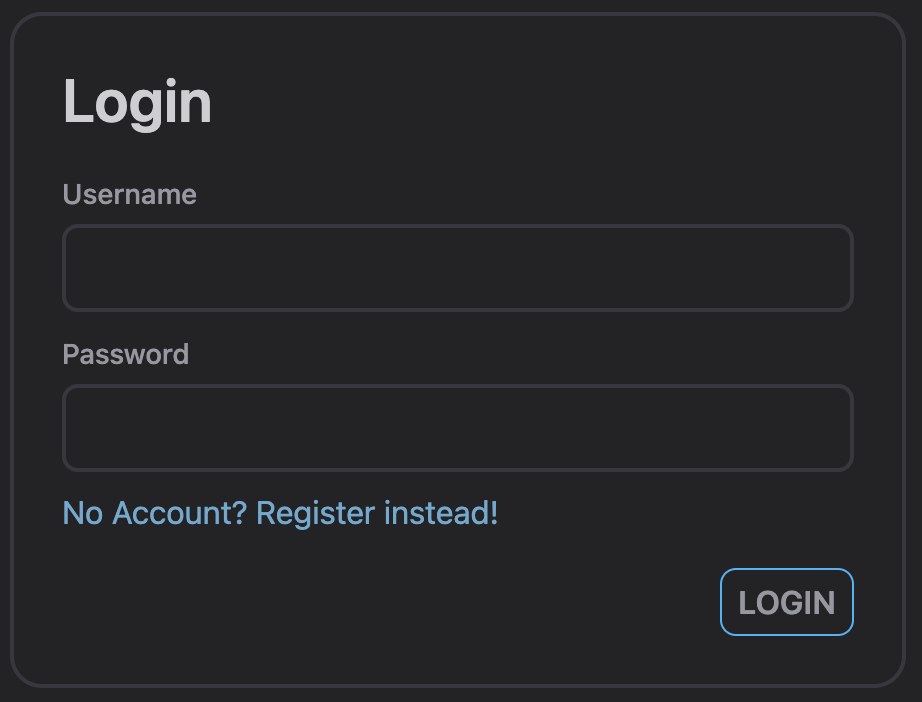
\includegraphics[scale=0.5]{./assets/login.png}
  \caption{Login-Form}\label{fig:loginForm}
\end{figure}

Eine weitere Funktionalität der Nutzerverwaltung ist, dass der Nutzer selbst
Anpassungen an ihrem Account machen können. Da nur sehr wenige Daten über den
Nutzer gespeichert werden, beschränkt dies sich auf drei Aktionen. So kann ein Nutzer
seinen Anzeigenamen für die Chats im Team bearbeiten können, welcher als Standard auf
den Nutzernamen gesetzt ist. Auch sollte es die Möglichkeit geben sein Passwort ändern zu können als auch den
Account endgültig zu löschen, wenn dieser nicht mehr benötigt wird. Diese
Optionen sollten über die Einstellungen zu finden sein.

\subsection{Teams}

Nachdem ein Nutzer in der Plattform eingeloggt ist, sollte dieser nun die
Möglichkeit haben, seine bisher erstellten Teams betrachten zu können und diese
zu verwalten. Hierfür wird zuerst den Benutzer über in einer Seitenleiste
alle seine Teams angeboten, welcher dieser selbst erstellt hat oder welche mit
ihm geteilt wurden. Über ein Modal, dass durch die Seitenleiste erreicht werden kann,
kann der Nutzer beide Aktionen durchführen. Zum Erstellen eines neuen Teams muss nur
der Name für dieses angegeben werden. Wenn einen bestehenden beigetreten werden sollte,
kann dies über einen Invite-Code erreicht werden.

\begin{figure}[ht]
  \captionsetup{justification=centering}
  \centering
  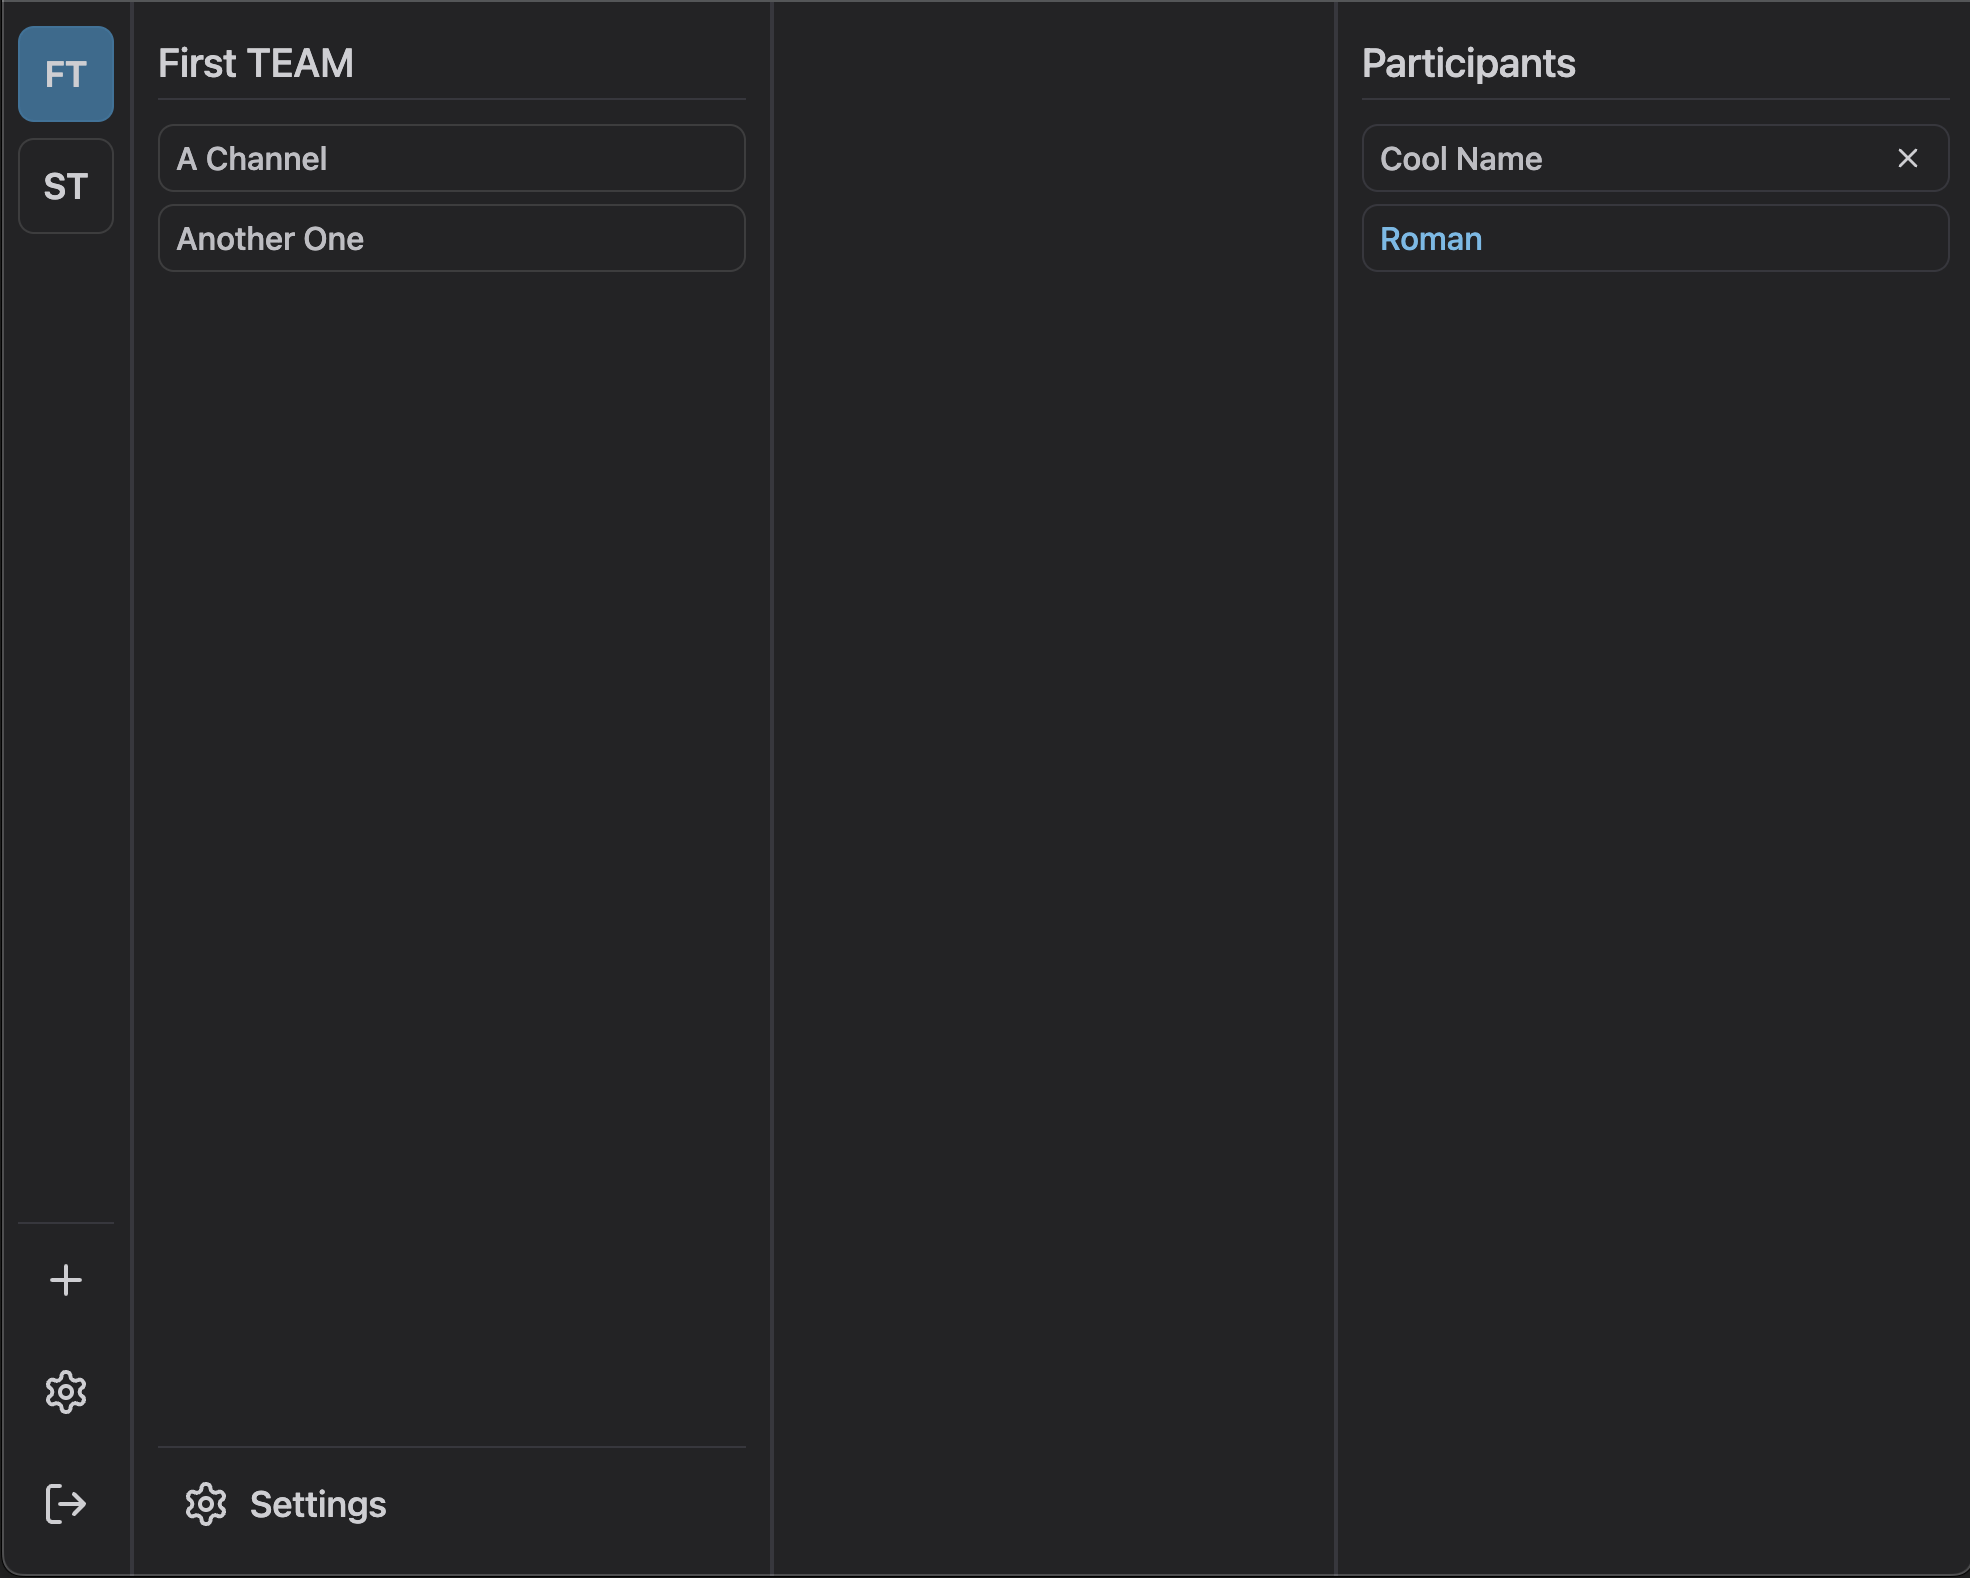
\includegraphics[scale=0.35]{./assets/team_overview.png}
  \caption{Teamübersicht}\label{fig:teamOverview}
\end{figure}

Von der Seitenleiste aus kann zu einem spezifischen Team navigiert werden, wo man zum dem
Hauptinterface der Applikation kommt. Diese ist eine drei geteilte Ansicht, welche die wichtigsten
Informationen für ein Team zeigt. Die Abbildung~\ref{fig:teamOverview} zeigt diese Ansicht. Diese
zeigt die bisher erwähnte Seitenleiste zur Übersicht aller Teams. Neben dieser finden sich zwei weitere
Seitenleisten, die zum Team gehören. In der linken Seitenleiste werden die Textkanäle angezeigt,
welche wenn betreten, visuell markiert werden. Neben dieser erhält der Besitzer des Teams einen Button
zu den Einstellungen eines Teams, während ein eigeladener Nutzer stattdessen einen Button zum Verlassen
des Teams auffindet. In der weiteren Seitenleiste finden sich alle Teilnehmer des Teams. Hier wird
der Besitzer des Teams speziell markiert. Auch erhält der Besitzer des Teams die Möglichkeit
über diese Liste eingeladene Nutzer aus dem Team zu entfernen.

Auch sollte jedes Team seine eigenen Einstellungen haben. In diesen Einstellungen sollen zuerst
allgemeine Optionen zu dem Team verwaltet werden. Dies beinhaltet zum bisherigen Zeitpunkt nur die Option
den Namen des Teams zu ändern. Daneben können hier die Textkanäle verwaltet werden. Dafür kann ein neuer
Kanal hinzugefügt und bestehende gelöscht werden. Die Option bestehende Kanäle nur umzubenennen, gibt es bisher nicht.
Zuletzt sollen hier neue Invite-Codes für das Team generiert werden. Dieser kann der Besitzer des Teams erstellen
und an weitere potentielle Nutzer geben, welche diese dann einlösen können. So ist eine einzelne Einladung nur
einmal gültig.

\subsection{Textkanäle}

Die letzte Funktionalität stellen die Textkanäle, mit den Nachrichten in diesen dar.
Wenn der Nutzer in einem Team zu einem Kanal navigiert, sollte dieser die Möglichkeit haben
einzelne Textnachrichten zu senden und bereits gesendete zu betrachten. Dafür wird ein Chatfenster
im bisher leeren Bereich zwischen den Seitenleisten, wie es in der Abbildung~\ref{fig:chatMessages} zu sehen ist,
im Team gezeigt, wenn auf einen der Kanäle in der Seitenleiste geklickt wird. Danach kann
der Nutzer Nachrichten schreiben, die allen Nutzern zugestellt werden. Wenn der Nutzer eine
Nachricht sendet und weitere Teilnehmer zurzeit denselben Kanal betrachten, wird diese Nachricht
allen Teilnehmern in Echtzeit zugestellt und die Seite muss nicht neugeladen werden. Neben den Echtzeit-Nachrichten kann auch die Historie des Kanales
mit den bisher gesendeten Nachrichten betrachtet werden. Diese sollten, damit der Nutzer nicht zu lange
auf die Historie warten muss, in kleinen Paketen geladen werden. Wenn der Nutzer an das Ende der bisher
geladenen Historie gescrollt hat, sollten diese falls noch Nachrichten vorhanden sind, nachgeladen werden.

\begin{figure}[ht]
  \captionsetup{justification=centering}
  \centering
  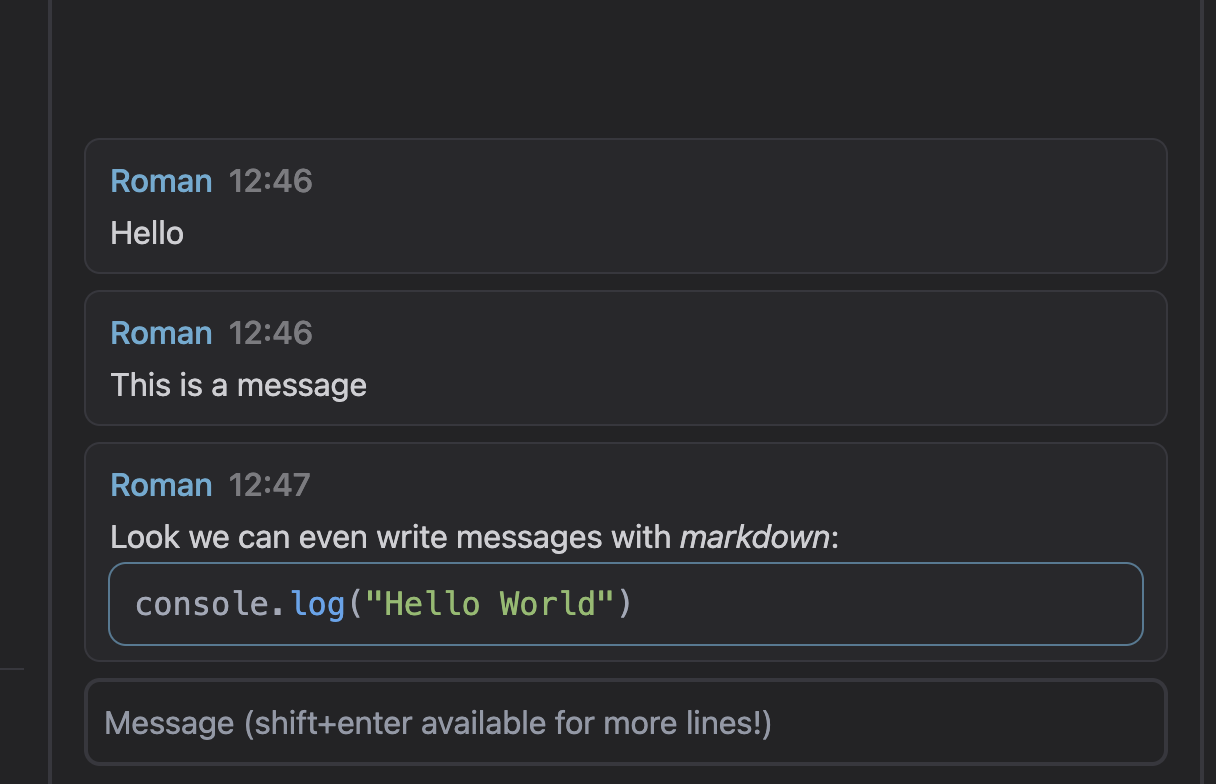
\includegraphics[scale=0.45]{./assets/chat_messages.png}
  \caption{Textkanalnachrichten}\label{fig:chatMessages}
\end{figure}

Um die Nachrichten zu schreiben, wird ein Textfeld angeboten. In diesem sollten die Nachrichten einfach
geschrieben werden und mit dem Drücken der Enter-Taste gesendet werden können. Da öfters auch längere
Nachrichten gesendet werden müssten, kann mit der Kombination aus der Shift- und Enter-Taste eine
neue Zeile begonnen werden. Das Textfeld wird sich hierfür auch automatisch in der Größe erweitern.

\section{Technologien}

Zuletzt sollen noch für die Konzeption die verwendeten Technologien, die
Architektur und das Datenmodell der Applikation beschrieben werden. Diese
sollen zeigen, nach welchen generellen Prinzipien das Projekt aufgebaut wurde.

\subsection{Datenmodell}

Da für dieses Projekt Nutzerdaten persistent gespeichert werden müssen, wird auch
ein Datenmodell für dieses benötigt. Dabei wurde für die persistente Haltung
der Daten sich für eine relationale Datenbank entschieden. Hierfür wurde die
Datenbank PostgreSQL verwendet. Die Abbildung~\ref{fig:dbSchema} zeigt dabei
das Datenbankschema der Applikation. Da die Tabellen im Backend direkt
auf Klassen gemapped werden und der Name beibehalten wird,
haben auch die Tabellen hier eine \anf{Entity}-Endung.


\begin{figure}[ht]
  \captionsetup{justification=centering}
  \centering
  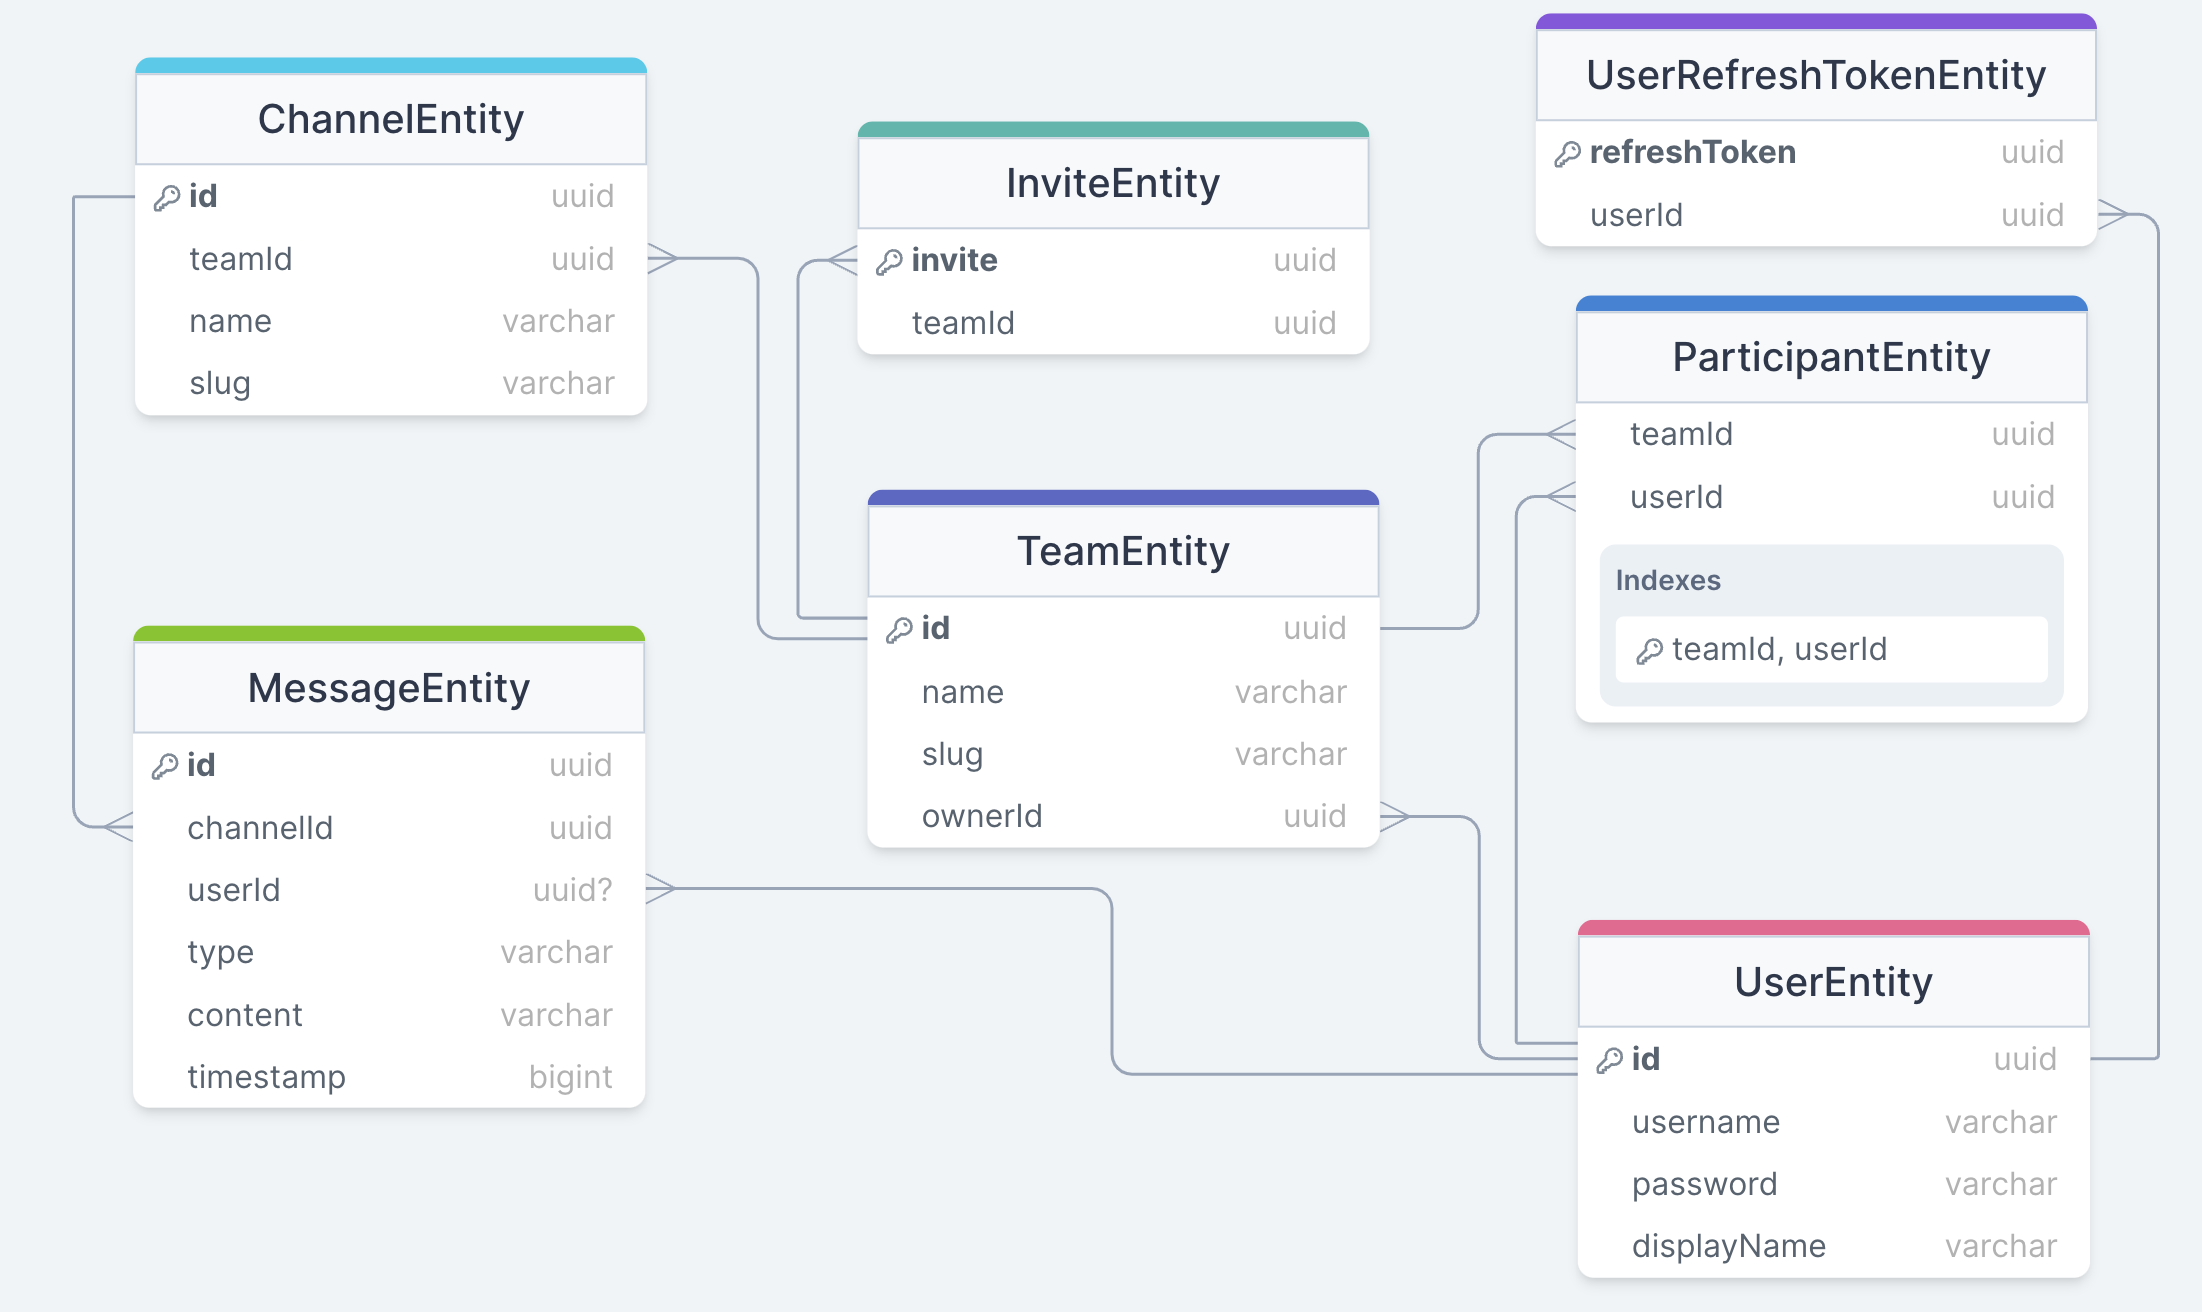
\includegraphics[scale=0.35]{./assets/db_schema.png}
  \caption{Datenbank-Schema}\label{fig:dbSchema}
\end{figure}

Für das Nutzerverwaltung werden zwei Tabellen benötigt, zum einen die
\emph{UserEntity} Tabelle als auch die \emph{UserRefreshTokenEntity} Tabelle.
Die \emph{UserEntity} Tabelle hält den Nutzer selbst. Dies beinhaltet den einen
Nutzernamen für den Login, ein Passwort, welches zuvor gehashed wird, und einen
Anzeigenamen für die Teilnehmerliste und Chatnachrichten. Die \emph{UserRefreshTokenEntity}
Tabelle wird zusätzlich benötigt, um die \emph{refreshTokens} für die spätere
Authentifikation zu speichern.

Die weiteren Tabellen werden zur Verwaltung der Teams und der Unterkomponenten gebraucht.
Die \emph{TeamEntity} Tabelle, speichert den Namen des Teams und einen \emph{slug},
welcher später im Browser für eine lesbare Identifikation in der URL verwendet wird. Ein
Team ist immer an einem Besitzer verknüpft. Um weitere Nutzer zu einem Team einzuladen,
werden die Einladungscodes in der \emph{InviteEntity} Tabelle gespeichert. Nach
einem erfolgreichen Beitritt zu einem Team wird die Zugehörigkeit über die \emph{ParticipantEntity}
Tabelle festgehalten, in der Nutzer zu Teams zugeordnet werden. Weiterhin die verschiedenen
Textkanäle in der \emph{ChannelEntity} Tabelle gespeichert und besitzen auch wie ein Team selbst,
\emph{slugs} für die Verwendung im Browser. Zuletzt gibt es noch eine Tabelle für die Textnachrichten.
In diesen wird der der Inhalt einer Nachricht, der Verfasser und ein Zeitstempel, wann die Nachricht
geschrieben wurde, persistiert. Für den Inhalt der Nachricht gibt es zwei Spalten die \emph{type}
und \emph{content} Spalte. Dies wurde dafür verwendet, um eine zukünftige Erweiterbarkeit vorzunehmen,
wo \zb{} auch neben einfachen Textnachrichten Bilder oder andere Nachrichtentypen gesendet werden können.

\subsection{Architektur}

Zur Entwicklung des Projektes wird noch die generelle Architektur für die
gesamte Applikation benötigt. Da es sich hier um eine Webapplikation handelt
wurde eine Client-Server-Architektur gewählt. Dies soll heißen, dass es einen
Server (im Folgenden auch \anf{Backend} genannt) gibt, welcher die Daten und
die Domänenlogik der Applikation hält. Dieser selbst bietet keine
Interaktivität für den Nutzer. Die Interaktivität kommt durch die einzelnen
Clients (im Folgenden auch \anf{Frontend} genannt), die die Nutzer bedienten
können Zustande. Da eine Webapplikation entwickelt wird, sind Clients die
Webbrowser der Benutzer. Ein Client bietet so die Interaktivität und
kommuniziert zum Erhalt der Daten und zur Manipulation dieser mit dem Server.

Der Server folgt dabei einer einfachen Schichtenarchitektur. In dieser werden
die Dienste einer Applikation in mehrere Schichten aufgebaut, welche aufeinander
aufbauen. So wird die Funktionalität der vorherigen Schicht verwendet, um diese
zu erweitern und eigene Funktionalität in einer hinzuzufügen.
(\vgl{}~\cite[\page{} 35]{layeredArch}) Dabei wurde das Backend in drei
Schichten gegliedert: die Datenschicht, die Businessschicht und die
Präsentationsschicht. Durch die Datenschicht werden wird ein Zugang zu den
Daten in der Datenbank und weiteren Persistenztechnologien ermöglicht.
Diese können durch die Schicht erhalten und manipuliert werden. In der Businessschicht
wird die eigentliche Applikationslogik erstellt. Dies beinhaltet \zb{} die Erstellung eines Nutzers
oder das Senden von Textnachrichten. Zuletzt bietet die Präsentationsschicht eine
REST-Schnittstelle für die Interaktivität des Frontends und eine zusätzliche Websocket-Schnittstelle,
um Echtzeit-Benachrichtigungen zu erhalten.

Das Frontend selbst wird durch eine Single Page Applikation (SPA) gebildet. In
dieser wird das User-Interface (UI) dynamisch komplett im Browser generiert.
Dafür wird eine minimale HTML-Datei ausgegeben, welche den gesamten Quelltext
für das Bilden des eigentlichen User-Interfaces und der Interaktion mit dem
Backend enthält. Der Client kann über asynchrone Request im Hintergrund Daten
vom Backend erhalten und die UI dementsprechend anpassen. Bei Aktionen des
Nutzers, wie \zb{} dem Erstellen eines neuen Projektes oder seinem Login,
können auch Anfragen an den Server gesendet werden, um diese auszuführen.

\subsection{Verwendete Technologien}

Zuletzt sollten in der Konzeption, die verwendeten Technologien für das Projekt
beschrieben werden. Hierfür wird zwischen dem Frontend und Backend
unterschieden, da dafür zwei verschiedene Programmiersprachen verwendet wurden.
Die verwendete relationale Datenbank für die Datenhaltung wurde dabei schon in
dementsprechenden Kapitel beschrieben.

Für die Entwicklung des Backends wurde die Programmiersprache Kotlin einer Sprache,
die auf der JVM verwendet werden kann, und deren Ökosystem verwendet. Die wichtigsten
Pakete waren hierfür: \emph{sqldelight}~\cite{sqldelight}, \emph{ktor}~\cite{ktor}
und \emph{dagger}~\cite{dagger} zusammen mit \emph{anvil}~\cite{anvil}. \emph{sqldelight}
bietet dafür einen Typsicheren Zugriff zur Datenbank, welche über Quelltext-Generation geschieht.
Durch \emph{ktor} konnte die REST-Schnitstelle als auch das Behandeln von Websocket-Verbindungen
für die Präsentationsschicht implementiert werden. Zuletzt konnte über die Bibliothek
\emph{dagger} und dem Erweiterungspaket \emph{anvil} Paket, eine automatische Dependency-Injection
für die Verbindung der einzelnen Schichten und deren Diensten ermöglicht werden.

Das Frontend wurde mithilfe von TypeScript und der UI-Bibliothek
\emph{SolidJS}~\cite{solidjs} entwickelt. Dabei handelt es sich um eine
komponentenbasierte UI-Bibliothek, durch die einzelne UI-Elemente mithilfe von
einfachen Funktionen beschrieben werden können. Neben dieser wurde zwei
kleinere Bibliothek, welche die Funktionalität von \emph{SolidJS} erweitern,
verwendet.

\chapter{Implementation}

Mit der beschriebenen Konzeption kann nun die Implementation des Webapplikation
besprochen werden. Diese wird dabei in das Frontend und Backend aufgeteilt. So
wurde zwar immer Feature basiert gearbeitet, \dh{} um eine Funktionalität zu
erweitern mussten meistens sowohl das Frontend als auch das Backend angepasst
werden, jedoch hat man eine starke Konzeptionelle Unterscheidung, wie beide
Applikationsteile aufgebaut sind. So sollen in den folgenden Abschnitten
zuerst das Backend und danach das Frontend beschrieben werden. Zuletzt soll noch eine
kurze Übersicht gegeben werden, wie die Webapplikation ausgeführt werden kann.

\section{Backend}

Das Backend wurde, wie schon in der Konzeption erläutert, mithilfe von der
Programmiersprache \emph{Kotlin} geschrieben und folgt einer
Schichtenarchitektur mit insgesamt drei Ebenen. Diese Schichten werden in den
folgendens Unterkapiteln näher betrachtet.

\subsection{Datenschicht}

Die Datenschicht soll es ermöglichen, einen Zugriff auf Daten von verschiedenen
Persistenz-Technologien zu erhalten und diese zu manipulieren. Dafür wurde hauptsächlich
mit der beschriebenen relationalen Datenbank PostgreSQL und der Bibliothek \emph{sqldelight}
gearbeitet. Durch diese Bibliothek konnte das Datenmodell und die Queries durch
SQL definiert werden und die Bibliothek generierte daraus Typsicheren Quelltext zur Interaktion
mit der Datenbank. Dafür müssen zuerst Migrationsdateien, welche einfache SQL-Skripte sind,
geschrieben werden. In diesen werden die üblichen Statements wie \code{CREATE TABLE}
das Datenmodell definiert. Daraus kann \emph{sqldelight} aus den definierten Tabellen einfache
Datenklassen zu den bilden. Separat werden auch noch die Queries für die Interaktion mit den Tabellen
definiert. Dafür werden Dateien erstellt aus denen \code{Query} Klassen generiert werden. In dieser
können Queries geschrieben werden, zu welchen immer ein Label gesetzt wird, welche den späteren
Methodennamen darstellt.

Mit der Quelltext-Generation konnte dann der \code{DatabaseService} geschrieben werden. In diesem
wird eine Verbindung über einen Connection-Pool zur Datenbank herstellt und mit der bestehenden Verbindung
die Query-Klassen initialisiert. Zusätzlich besteht ein \code{MigrationService}, der im \code{DatabaseService}
genutzt wird. So müssten die bereits in SQL geschriebenen Migrationen auch ausgeführt werden, und die bisherige
Version des Datenbankschemas persistiert werden. \emph{sqldelight} generiert dafür eine \code{migrate}-Methode,
die die Migrationen ausführt. Für diese muss aber die bisherige Version des Datenbankschemas übergeben werden.
Dafür wird im \code{MigrationService} eine Tabelle in der Datenbankerstellt, welche die Version persistiert.
So kann diese Version für die Migration erhalten werden und nach der Migration auf die neueste Version gesetzt werden.

Neben der Datenbank wird noch im Backend der geteilter In-Memory-Cache \emph{redis}~\cite{redis} eingesetzt.
Damit können Daten geteilt bei mehreren Backend-Instanzen zwischengespeichert werden. Dies wurde verwendet um
Datenbankabfragen, welche eine längere Zeit dauern zwischenzuspeichern und die Ergebnisse schneller zurückgeben
zu können. Ein Beispiel ist hierfür der \code{AuthorizationCache}, in welcher die Zugriffsberechtigungen für
das Absichern der API zwischenspeichert.

\subsection{Businessschicht}

Mit dem rohen Datenzugriff kann nun die eigentliche Applikationslogik für das
Backend erstellt werden. Dies erfolgt in den \emph{Services} Klassen, welche
auf den \emph{Queries} und \emph{Caches} der vorherigen Schicht aufbauen. Diese enthalten die
spezifischen Applikationslogik, um \zb{} die Aktionen für die Teams oder der
Authentifikation durchzuführen. Diese Services haben dabei keinen
internen Zustand und hängen nur von der Datenhaltung oder weiteren Services ab.

Die Services für den Nutzer, die Teams, die Team-Kanäle und die Team-Teilnehmer, bieten dabei
eine sehr ähnliche Schnittstelle an. Diese hauptsächlich ein Create-Read-Update-Delete (CRUD)
Interface an, um eines oder mehrere Datensätze zu erhalten, neue zu erstellen
oder alte zu verändern und zu löschen. Es gibt auch spezifischere Aktionen auf den jeweiligen
Daten, welches \zb{} welches mehr als nur die Manipulation eines Objektes
erfordert. Dafür werden domänenspezifische Aktionen angeboten. Ein Beispiel ist das Beitreten
eines neuen Teammitgliedes zu einem Team. Hier werden auch die Daten aus der Persistenz-Schicht
zu domänenspezifischen Objekten umgewandelt, welche auch für die spätere Präsentationsschicht
serialisierbar sind.

So gibt es aber auch Services, die nicht in das CRUD-Schema passen. Dies ist
\zb{} der \code{AuthenticationService} oder \code{AuthorizationService}, welche die Nutzer Authentifikation und
Autorisation steuert. Über den \code{Authentication\-Service} können Nutzerkonten
über eine Registration erstellt werden. Um den Nutzer für die spätere Authentifikation zu
identifizieren wird eine Kombination aus einem kurzlebigen Access-Token und
einem langlebigen Refresh-Token verwendet. Der Access-Token, ist dabei ein
signierter \emph{JWT} Token, welcher nur eine kurze Gültigkeit von einem Tag
hat. Dieser wird zu der eigentlichen Authentifikation verwendet. Wenn der
bisherige Access-Token abgelaufen ist, kann der Refresh-Token verwendet werden,
um einen neuen AccessToken generieren zu lassen. Dafür muss der Refresh-Token
in der Datenbank gespeichert werden. Durch diese Kombination beider Tokens, muss
nur selten ein Datenbankzugriff zur Authentifikation erfolgen. Zuletzt hat der
\code{AuthorizationService} Methoden zur Autorisation. Mit diesen kann geprüft werden,
ob ein Nutzer der Besitzer eines Projektes ist oder dieses für ihn geteilt
wurde, womit in der Präsentationsschicht die API-Routen abgesichert werden können.

Das das Backend über eine Echtzeit-Komponente für Chats der einzelnen Teams und zur
generellen Benachrichtigung von Events verfügt, gibt es noch \emph{Services} zur Steuerung
von diesen. Um auch hier eine Skalierung des Backends zu ermöglichen, wurde das Pub-Sub-System \emph{Nats}~\cite{nats}
eingesetzt. Mit diesem System ist es möglich sich für verschiedene Nachrichtenkanäle zu registrieren,
und beim Senden von Nachrichten davon benachrichtigt werden. So kann \zb{} bei mehreren
Backend-Instanzen eine Instanz für den Client eine Chat-Nachricht senden und alle weiteren
Backends würden davon benachrichtigt werden. Das wird verwendet, da die Websocket-Verbindungen
zwar zustandsvoll sind und so immer an ein Backend gebunden sind, jedoch mit dieser Technik
Benachrichtigungen, immer an alle Clients ausgeliefert werden können, egal mit welcher spezifischen
Instanz, diese sich verbunden haben.

\subsection{Präsentationsschicht}

Als letzte Schicht wird noch die Präsentationsschicht betrachtet. Diese bietet
eine REST-Schnittelle durch die Bibliothek \emph{ktor} an. Zum Erstellen von
API-Routen wurden Klassen erstellt, welche das selbst geschrieben \code{HttpRouter}
Interface implementieren. In diesem wird ein Callback erfüllt, über welchen die einzelnen
API-Routen registriert werden können. Für jede Route wird so in der Klasse eine
Handler-Methode geschrieben. In dieser Methode stehen einen die verschiedenen
HTTP-Request Daten zur Verfügung. So kann in den Methoden \zb{} ein JSON-Objekt aus dem
HTTP-Body der Abfrage deserialisiert werden. Mit dem erhaltenen Daten können dann
die Methode der Services aufgerufen, die erhaltenen domänenspezifischen Objekte
in JSON-Objekte serialisiert und diese darauf als Antwort dem Client zurückgegeben werden.
Die implementierten \code{HttpRouter} konnten dann dem \code{HttpService} übergeben werden,
wo der Http-Server von \code{ktor} gestartet wurde um den Router-Klassen konfiguriert  wurde.

\subsection{Dependecy Injection}

Für eine automatische Instanziierung aller benötigter Klassen und eine passende
Anbindung derer Abhängigkeiten, wurde die Dependency-Injection Bibliotheken
\emph{dagger} und \emph{anvil} verwendet. Für die Integration in die bisher beschriebenen
Klassen müssen hierfür nur um Annotationen ergänzt werden. Dadurch wird mitgeteilt, über welchen
Konstruktor \zb{} die Klasse initialisierbar ist.

Zum Erstellen und Initialisieren des gesamten Abhängigkeits-Graphen der Applikation stellt der \code{AppComponent}
den Einttritspunkt dar. Für dieses erstellt \emph{dagger} den gesammten Injektions-Quelltext, um
eine konkrete Instanz des \code{AppComponents} zu erhalten. In diesem ist der \code{ServiceManager}
vorhanden, welcher die Dienste der Applikation verwaltet und startet.

\section{Frontend}

Nun sollte auch das Frontend der Applikation beschrieben werden, welches mit
der Programmiersprache \emph{TypeScript} und der UI-Bibliothek \emph{SolidJS}
entwickelt wurde. Das Frontend hat dabei die Aufgabe, Daten von dem Backend zu
erhalten und daraus eine Interaktive-Nutzeroberfläche im Browser zu erstellen.
Auch sollten bei Nutzerinteraktionen die Daten des Backends manipuliert werden
können. Dafür kann das Frontend in zwei Teile gegliedert werden: Die
UI-Komponenten, welche die UI und deren Interaktivität bilden und den
dazugehörigen Zuständen, welche die Daten zur Darstellung und Methoden für die
Datenmanipulation für die UI-Komponenten anbieten.

Da die einzelnen Zustände die Grundlage für die UI-Komponenten bilden, sollten
sich diese zuerst betrachtet werden. Da \emph{SolidJS} eine reaktive
UI-Bibliothek ist, werden für das Bilden von Zuständen, primitive
Datenstrukturen angeboten, mit welchen die UI-Komponenten angepasst werden
können, falls sich der Inhalt der Datenstrukturen ändern. Ein Beispiel ist
dafür die \code{createSignal} Funktion. Die einen Getter für den Erhalt der
Daten und einen Setter zum Setzen neuer Daten zurückgibt. Wenn ein neuer Wert
über den Setter gesetzt wird, wird jede Komponente, die den Getter verwendet
mit dem neuen Inhalt angepasst. Solche primitive werden nun in
\emph{State}-Klassen verwendet, um den Zustand für die UI zu bilden. Dafür
halten diese zum einen den Zustand für die UI-Logik, wie \zb{} den Zustand
einer Form für das Erstellen das Verwalten eines Teams. Auch halten die States, die aus dem
Backend erhaltenen Daten. Die Zustandsklasse bietet nun eine Schnittstelle
durch Methoden an, um die internen Daten zu erhalten und zu verändern.

Diese Zustände werden verwendet, um die UI zu bilden und eine Interaktivität zu
dieser hinzuzufügen. Dafür werden in \emph{SolidJS} \sog{} Komponenten
verwendet, welche einfache Funktionen sind, die HTML-Markup oder andere
Komponenten zurückgeben können. Diese werden im Vergleich zu anderen
Komponentenbasierten UI-Bibliotheken nur einmal für das Rendern aufgerufen. So
kann hierarchisch die gesamte Applikation gebildet werden. Die Komponenten sind
dabei nach den möglichen Navigations-Routen der Applikation organisiert. Diese
können in der \code{App} Komponenten zu der Applikation über einen Routing
Mechanismus eingebunden werden. So gibt es immer für jede mögliche Destination
eine \code{Route} Komponente, die über diese Route verantwortlich ist. Dabei
können auch Routen weitere Routen selbst erhalten. So ist \zb{} die Route
für ein einzelnes Team in der Route für die gesamte Applikation eingebunden.
So werden wie die Komponenten selbst, die Routen hierarchisch angeordnet In
diesen Routen werden auch immer die passenden Zustände aus dem vorherigen Abschnitt
gebildet. Alle weiteren Komponenten unter einer \code{Route} können dabei den Zustand
von der Route erhalten, um mit den Daten die UI zu bilden oder die Interaktivität
der UI zu geben.

\section{Inbetriebnahme}

Zuletzt sollte noch beschrieben werden, wie das Projekt gestartet werden kann.
Hierfür können werden zwei Möglichkeiten geboten. So kann man hierfür zum einen
die lokale Entwicklungsvariante verwenden. In dieser müssen das Frontend und
Backend separat gestartet werden. Eine genaue Anleitung findet sich in der
\code{README} Datei im Root des Projektes. Hierbei kann mit der Entwicklungsumgebung
\emph{Intellij IDEA} das Backend gestartet werden. Das Frontend hingegen benötigt,
dadurch dass es in \emph{TypeScript} geschrieben wurde, eine relativ neue Version von
\emph{Node.js}~\cite{node} und der Paket-Manager \emph{pnpm}~\cite{pnpm}.
Diese Variante kann verwendet werden, um das Projekt auszuführen jedoch sollte dafür
wegen der Einfachheit die nächste Variante verwendet werden.

Eine weitere Möglichkeit, das Projekt in Betrieb zu nehmen, ohne die gesamten
Abhängigkeiten für das Frontend und Backend zu installieren, ist das Container
Orchestrierungstool \emph{Docker}~\cite{docker}. Dafür wird nur \emph{docker}
selbst und das Tool \emph{docker-compose} benötigt, welches bei den älteren
Versionen von \emph{docker} seperat installiert werden muss. Dafür findet sich
im Root des Projektes eine \code{compose.yml} Datei. In dieser wird das
Backend und Frontend neben den Persistenz-Technologien gestartet. Hierbei sollten
noch Konfigurationsdateien erstellt werden. Dafür braucht es im Root des Projektes
eine \code{.env} und eine \code{config.json} Datei. Auch hierfür findet sich in der \code{README}
Datei des Projektes eine genaue Anleitung, wie mit welchen Daten diese Dateien befüllt werden sollten.
Danach kann das Projekt mit den \code{docker-compose up ----build} Befehl gestartet werden.

\chapter{Fazit}

Nach der Beschreibung des Projektes sollte noch ein kurzes Fazit zum Projekt
selbst und der erstellten Applikation gegeben werden. So war es für dieses
Projekt möglich eine vollwertige Webapplikation für das die asynchrone Kommunikation
in Teams zu erstellen. So konnten alle wichtigen Komponenten wie die Nutzerverwaltung,
das Arbeiten mit den Teams und deren Kanälen und ein Echtzeit-Benachrichtigung-System
für die Textnachrichten und weitere Events implementiert werden. Insgesamt kann das
Projekt als Erfolg betrachtet werden.

Durch das Projekt konnte für mich perönlich gezeigt werdem, wie effektiv mit der
Programmiersprache Koltin Backends erstellt werden können. So wird im Vergleich
die Ergonomie zu der Programmiersprache Java verbessert, wobei sich diese auch in den
letzten Java Versionen verbessert hat. Auch können alle bisher geschriebenen Bibliotheken
für die JVM, wie \zb{} die für \emph{redis} oder \emph{Nats} einfach Verwendet und
integriert werden.

Eine weitere wichtige Entscheidung, ohne die ein hohes Maß an Interaktivität in
der Applikation schwierig gewesen wäre, war die Erstellung einer SPA. So musste
nicht das Templating der HTML-Dateien vom Backend übernommen werden. Dadurch
konnten einfach mit Hilfe von \emph{SolidJS} dynamische Anwendungen mit einem
hohen Maß an Interaktivität erstellt werden, wecher auch ihre Daten dank einer
Websocket-Verbindungn in Echtzeit anpassen können.

Zum Abschluss kann gesagt werden, dass mir die Entwicklung des Projektes eine
große Freude bereitet und einen tieferen Einblick in die Webentwicklung gegeben
hat.


\appendix
\printbibliography{}

\end{document}
